% $Header$

\documentclass{beamer}
\mode<presentation>
{
	\usetheme{Madrid}
	% or ...
	
	\setbeamercovered{transparent}
	% or whatever (possibly just delete it)
}
\usepackage[english]{babel}
% or whatever

\usepackage[latin1]{inputenc}
% or whatever
\usepackage[T1]{fontenc}
\usepackage[cache=false]{minted}
\usepackage{tikz}
\usetikzlibrary{decorations.pathreplacing}
% Or whatever. Note that the encoding and the font should match. If T1
% does not look nice, try deleting the line with the fontenc.

\makeatother
\setbeamertemplate{footline}
{
	\leavevmode%
	\hbox{%
		\begin{beamercolorbox}[wd=.4\paperwidth,ht=2.25ex,dp=1ex,center]{author in head/foot}%
			\usebeamerfont{author in head/foot}\insertshortauthor
		\end{beamercolorbox}%
		\begin{beamercolorbox}[wd=.6\paperwidth,ht=2.25ex,dp=1ex,center]{title in head/foot}%
			\usebeamerfont{title in head/foot}\insertshortdate\hspace*{3em}
			\insertframenumber{} / \inserttotalframenumber\hspace*{1ex}
	\end{beamercolorbox}}%
	\vskip0pt%
}
\makeatletter
\setbeamertemplate{navigation symbols}{}

\title[Ray Tracing] % (optional, use only with long paper titles)
{3D Rendering with Ray Tracing}

\author{Calvin Godfrey}

\institute[] % (optional, but mostly needed)
{Virginia Polytechnic Institute and State University}

\date[https://github.com/calvin-godfrey/RenderingWorkshop]{??? February 2021}
\subject{Talks}

\AtBeginSection[]
{
	\begin{frame}
	\frametitle{Table of Contents}
	\tableofcontents[currentsection]
\end{frame}
}

\begin{document}

\begin{frame}
	\titlepage
\end{frame}

\section{About Me}

\begin{frame}
	\frametitle{About Me}
	\begin{itemize}
		\item Junior at Virginia Tech
		\item Began ray tracing in late April
	\end{itemize}
	\begin{columns}[T]
		\begin{column}{0.5\textwidth}
			\centering
			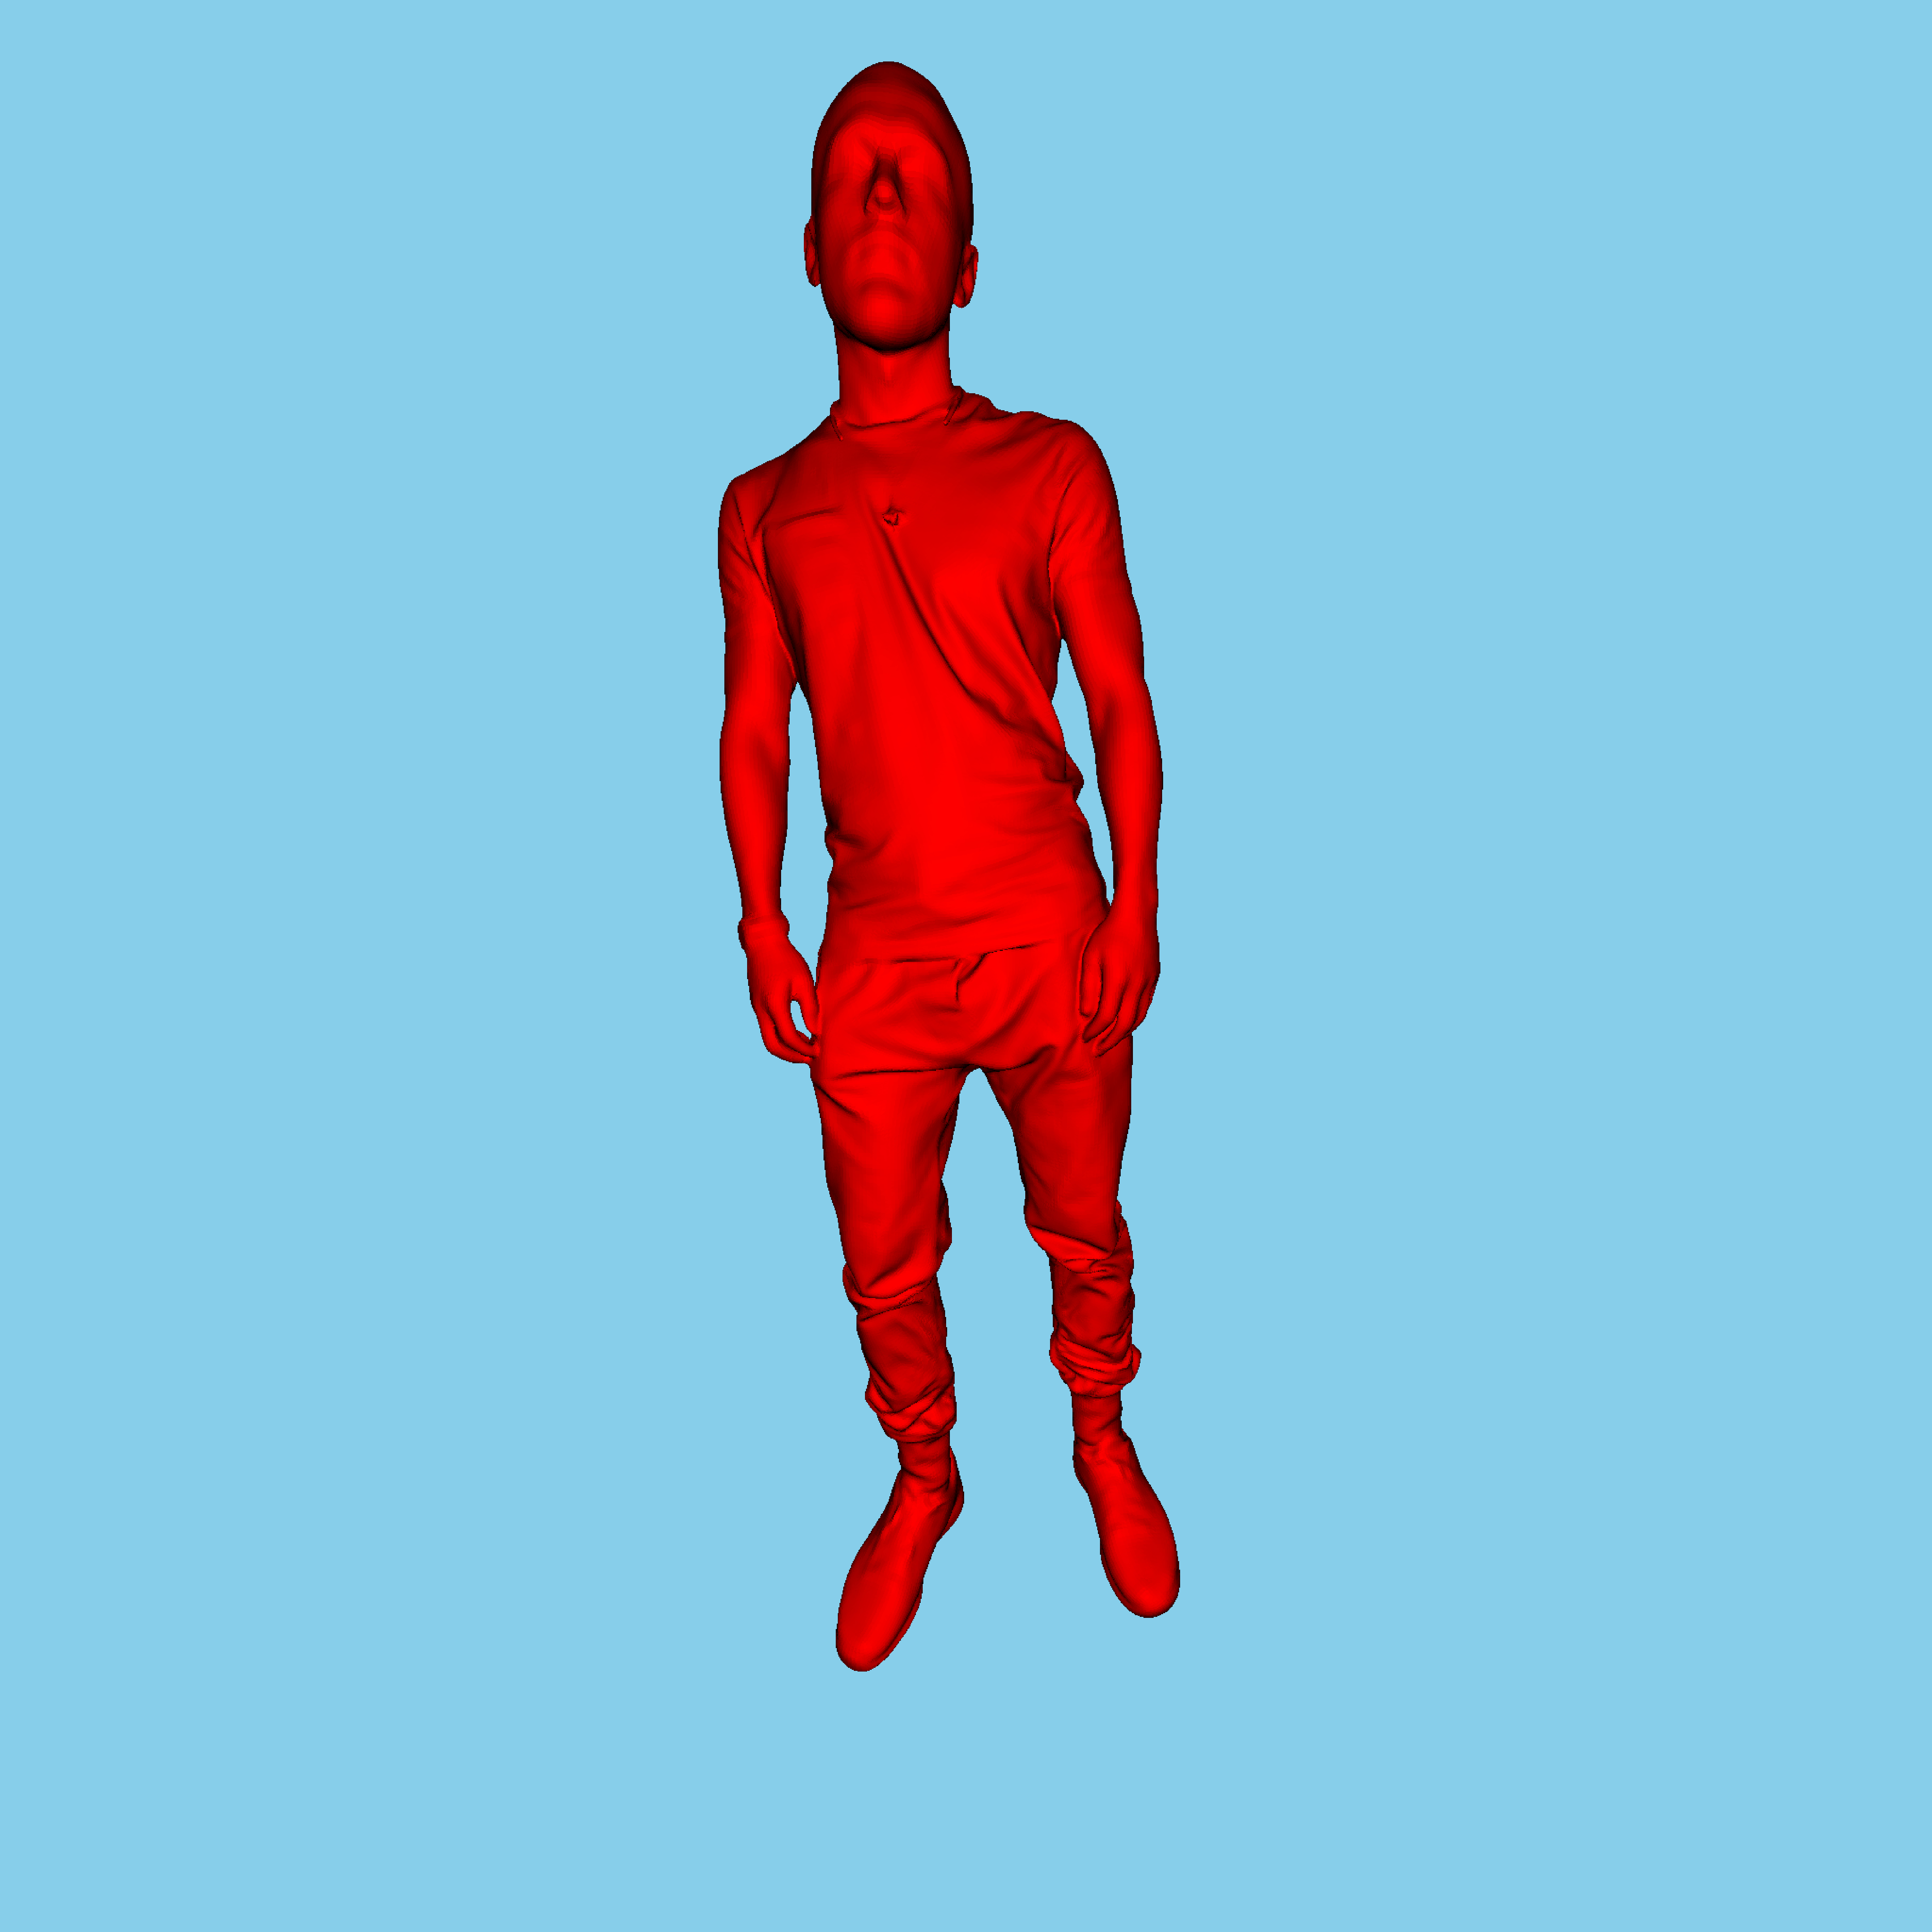
\includegraphics[width=\textwidth]{media/person.jpg}

			\textit{Rendered in June; 11 hours}
		\end{column}
		\begin{column}{0.5\textwidth}
			\centering
			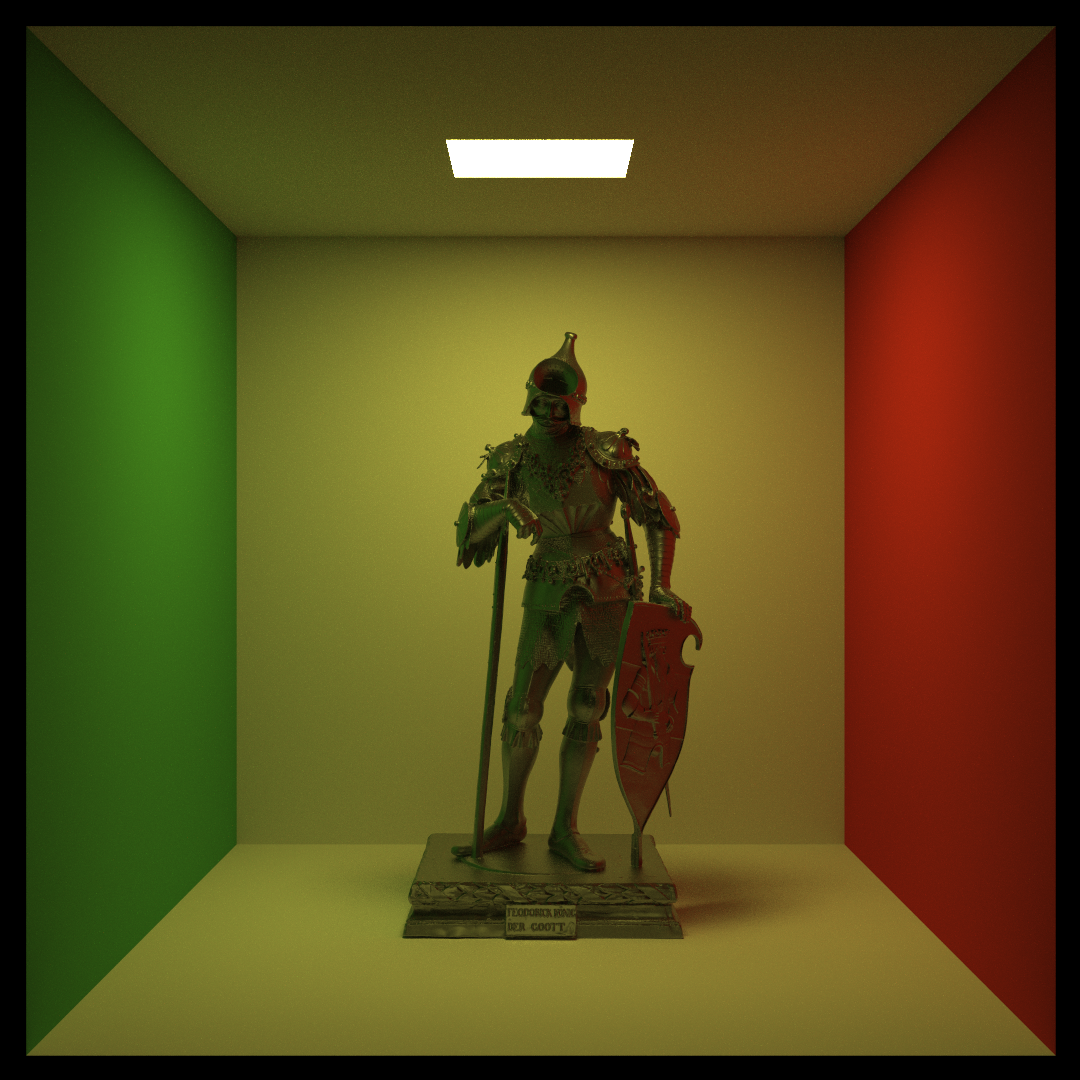
\includegraphics[width=\textwidth]{media/statue.png}

			\textit{Rendered in December; 2.5 hours}
		\end{column}
	\end{columns}
\end{frame}

\section{Intro to Computer Graphics}

\begin{frame}
	\frametitle{Computer Graphics}
	\begin{itemize}
		\item<1-| alert@1> Software Rasterization
		
		\only{
			\begin{center}
				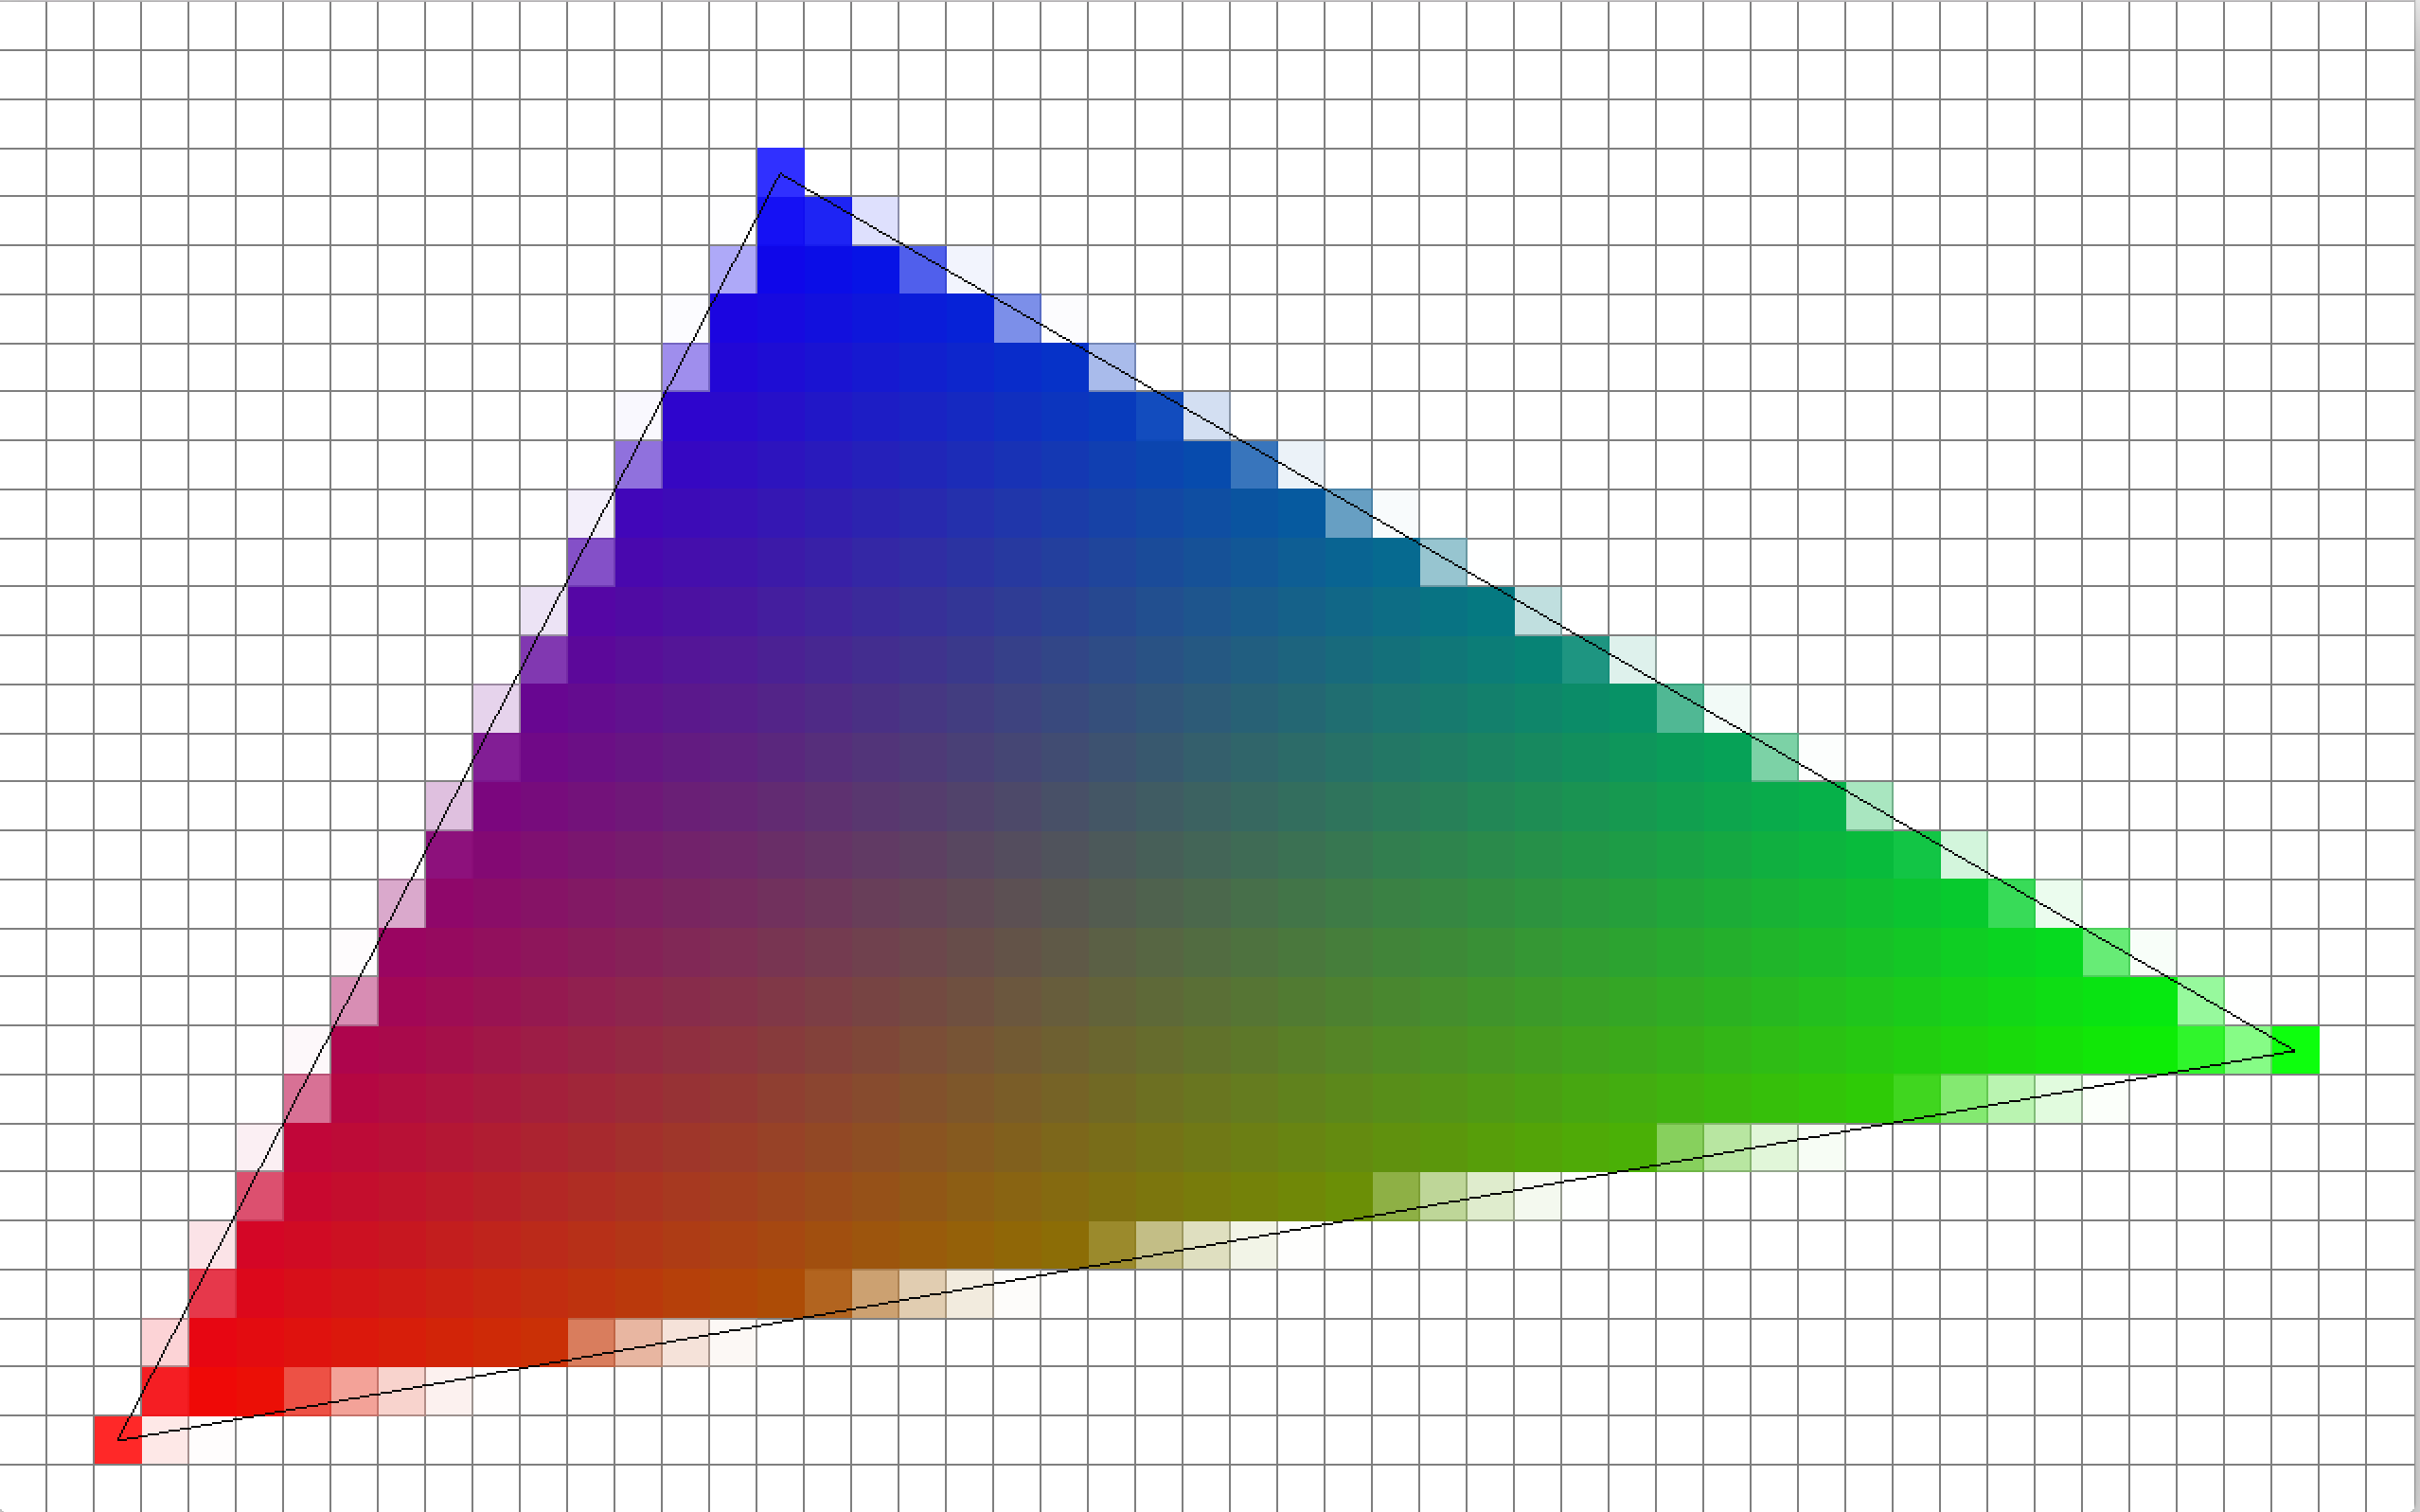
\includegraphics[width=0.4\textwidth]{media/Rasterization.png}
			\end{center}
			
			\begin{itemize}\color{black}
				\item ``Given \textit{shape}, what pixels should show this?''
				\item Faster, commonly used in cartoon-styled games
				\item Not the focus of this workshop
			\end{itemize}
			}<1>
		\item<2-| alert@2> Ray Tracing
	\end{itemize}
	\only{
		\centering
		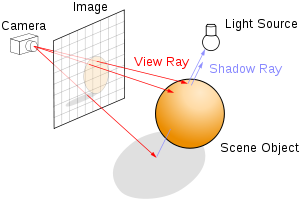
\includegraphics[width=0.4\textwidth]{media/raytracing.png}
		\begin{itemize}
			\item ``Given \textit{pixel}, what object should this show?''
			\item Slower, but more realistic
			\item Involves the study of physics (light interactions), math (sampling techniques) and computer science (acceleration structures)
		\end{itemize}
	}<2>
\end{frame}

\section{Provided Code}

\begin{frame}[fragile]
	\frametitle{Vector}
	\begin{minted}{python}
class Vector3:
    def __init__(self, x, y, z):
        self.x, self.y, self.z = x, y, z
	\end{minted}
	\begin{itemize}
		\item Standard vector operations; addition and scalar multiplication
		\item Also contains utility functions for dot/cross product, length, normalize, etc.
		\item Used to represent points, vectors, and colors
	\end{itemize}
\end{frame}

\begin{frame}[fragile]
	\frametitle{Ray}
	\begin{minted}{python}
class Ray:
    def __init__(self, origin, direction):
        self.origin = origin
        self.direction = direction
        
    def at(self, t):
        return self.orgin + t * self.direction
\end{minted}
	\begin{itemize}
		\item Contains origin of ray and direction (both \texttt{Vector3})
		\item Includes method to find point at given distance on ray
	\end{itemize}
\end{frame}

\begin{frame}
	\frametitle{ImageWrapper}
	\inputminted{python}{scripts/wrapper.py}
	\begin{itemize}
		\item Constructor takes file name and file size
		\item Provides method to save file and write pixel at specified coordinate
	\end{itemize}
\end{frame}

\section{Implementing new Code}

\begin{frame}
	\frametitle{Camera}
	\begin{columns}[T]
		\begin{column}{0.5\textwidth}
			\begin{center}
				\begin{tikzpicture}[scale=0.8]
					\tikzset{>=stealth}
					% special method of noting the position of a point
					\draw (0, 0) coordinate (P) node [above left] {};
					\node at (P) {\textbullet};
					\path[draw] (3.4641, -2) -- (3.4641,2);
					\path[draw] (P) -- (3.4641, 2);
					\path[draw] (P) -- (3.4641, -2);
					\draw (0.55, 0) node [right] {$\theta$};
					\draw[black] (0.526646, -0.304059) arc (-30:30:0.60811858);
					\draw (3.4, 0) node [right] {$h$};
					\draw [decorate, decoration={brace,amplitude=5pt,mirror}]
					(0, -2.3) -- (3.4641, -2.3) node[midway,yshift=-3em] {$d$};
				\end{tikzpicture}
			\end{center}
		\end{column}
		\begin{column}{0.5\textwidth}
			\only{
				\begin{itemize}
					\item Requires location, view direction (target), and orientation (`up' direction), field of view, and aspect ratio
					\item Constructor calculates useful information about plane
				\end{itemize}
			}<1>
			\only{
				\begin{itemize}
					\item Given \texttt{vfov} of $\theta$ and focal distance $d$, $h=2d\tan\left(\frac\theta2\right)$
					\item Width of plane is $h$ multiplied by aspect ratio of image
					\item Constructor also calculates location of bottom-left corner; used in later methods
				\end{itemize}
			}<2>
		\end{column}
	\end{columns}
\end{frame}

\begin{frame}[fragile]
	\frametitle{Camera}
	\begin{itemize}
		\item First, find basis vectors for camera
	\end{itemize}

	\inputminted[fontsize=\footnotesize]{python}{scripts/cameraConst1.py}
\end{frame}

\begin{frame}[fragile]
	\frametitle{Camera}
	\begin{itemize}
		\item Then define size of the plane
	\end{itemize}

	\inputminted[fontsize=\footnotesize]{python}{scripts/cameraConst2.py}
\end{frame}

\begin{frame}[fragile]
	\frametitle{Camera}
	\begin{itemize}
		\item Finally, store the lower-left corner of plane
	\end{itemize}

	\inputminted[fontsize=\footnotesize]{python}{scripts/cameraConst3.py}
\end{frame}

\begin{frame}[fragile]
	\frametitle{Camera Ray Generation}
	\begin{itemize}
		\item Given $(x, y)\in [0, 1)^2$, return ray going through that point in plane
	\end{itemize}
	\only{
		\begin{center}
			\begin{tikzpicture}[scale=0.8]
			\path[draw] (0, 0) -- (10, 0) -- (10, 6) -- (0, 6) -- (0, 0);
			\node at (0, 0) {\textbullet};
			\draw (0, 0) node [below left] {Bottom-left corner};
			\node at (7, 3) {\textbullet};
			\draw (7, 3) node [below right] {$(x, y)$};
			\draw[dashed] (7, 0) -- (7, 3) -- (0, 3);
			\draw[thick,->] (-0.2, 0) -- (-0.2, 6);
			\draw[thick,->] (0, -0.2) -- (10, -0.2);
			\end{tikzpicture}
		\end{center}
	}<1>
	\begin{onlyenv}<2>
		\inputminted{python}{scripts/cameraGen.py}
	\end{onlyenv}
\end{frame}

\begin{frame}[fragile]
	\frametitle{Main Rendering Loop}
	\begin{itemize}
		\item First, define constants, \texttt{Camera}, and \texttt{ImageWrapper}
	\end{itemize}
	\inputminted[fontsize=\footnotesize]{python}{scripts/mainLoop1.py}
\end{frame}

\begin{frame}[fragile]
	\frametitle{Main Rendering Loop}
	\begin{itemize}
		\item Then iterate over each pixel and calculate color
	\end{itemize}
	\inputminted[fontsize=\footnotesize]{python}{scripts/mainLoop2.py}
\end{frame}

\begin{frame}[fragile]
	\frametitle{First Render Test}
	\begin{itemize}
		\item Set color of pixel depending on $z$ component of ray's direction
	\end{itemize}
	\begin{onlyenv}<1>
		\inputminted{python}{scripts/firstRender.py}
	\end{onlyenv}
	\only{
		Resulting image:
		\begin{center}
			
\includegraphics[width=0.5\textwidth]{media/firstRender.png}
		\end{center}
	}<2>
\end{frame}

\section{Shapes and Intersections}

\begin{frame}
	\frametitle{Sphere-Ray Intersection}
	\only{
		\begin{itemize}
			\item Given ray with origin $O$ and direction $D$, where does it first intersect a sphere with center $C$ and radius $R$?
			\item Equivalent question is intersection between ray at $O-C$ and direction $D$ and sphere centered at origin with radius $R$
			\begin{itemize}
				\item Parameterize ray as $(O-C) + tD$; each value of $t$ gives new point $P$ on ray
				\item $P$ is on sphere if $P^2 = R^2$, or $P^2 - R^2 = 0$.
				\item But $P=(O-C) + tD$, giving the following equation:
			\end{itemize}
		\end{itemize}
		$$|(O - C) + tD|^2 - R^2 = 0$$
	}<1>
	\only{
		\begin{align*}
			|(O - C) + tD|^2 &= R^2 \Longleftrightarrow \\ 
			((O-C)+tD)\cdot ((O-C)+tD) &= R^2 \Longleftrightarrow \\
			O\cdot O - 2O\cdot C + 2t(O\cdot D) + C\cdot C - 2t(C\cdot D)+ t^2(D\cdot D) &= R^2 \Longleftrightarrow \\
			(D\cdot D)t^2 + (2O\cdot D - 2C\cdot D)t + O\cdot O + C\cdot C - 2O\cdot C &= R^2 \Longleftrightarrow \\
			(D\cdot D)t^2 + 2D\cdot (O - C) t + (O - C) \cdot (O - C) - R^2 &= 0
		\end{align*}
		
		where $\cdot$ indicates the dot product between two vectors
		\begin{itemize}
			\item This is a quadratic equation in $t$ with $a=D\cdot D$, $b=2D\cdot (O-C)$, and $c=(O-C)\cdot (O-C) - R^2$
			\item Two solutions to quadratic formula give two (possible) intersection points
		\end{itemize}
	}<2>
\end{frame}

\begin{frame}
	\frametitle{Geometric Interpretation of Ray-Sphere Formula}
	\begin{itemize}
		\item Two real solutions: Ray intersects with sphere twice
		\begin{itemize}
			\item Two positive solutions: Two intersections ``in front'' of ray (example 1 below)
			\item One positive, one negative solution: Ray starts within sphere (example 3)
			\item Two negative solutions: Sphere is ``behind'' ray (example 5)
		\end{itemize}
		\item One solution: Ray ``grazes'' sphere at single point (example 2)
		\item No real solution: Ray misses sphere (example 4)
	\end{itemize}
	\begin{center}
		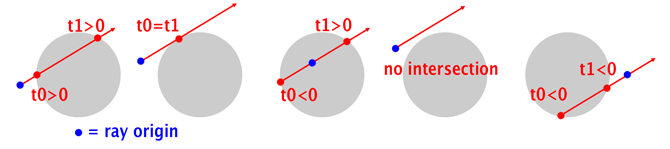
\includegraphics[width=0.7\textwidth]{media/sphereIntersection.png}
	\end{center}
\end{frame}

\begin{frame}[fragile]
	\frametitle{Quadratic Formula Solver}
	\inputminted{python}{scripts/quadratic.py}
\end{frame}

\begin{frame}[fragile]
	\frametitle{Sphere-Ray Intersection}
	\inputminted{python}{scripts/sphereIntersection.py}
\end{frame}

\begin{frame}[fragile]
	\frametitle{Rendering a Sphere}
	\begin{itemize}
		\item Now update the render loop from earlier to use this
	\end{itemize}
	\begin{onlyenv}<1>
		\inputminted{python}{scripts/sphereRender.py}
	\end{onlyenv}
	\only{
		And the new result:
		\begin{center}
			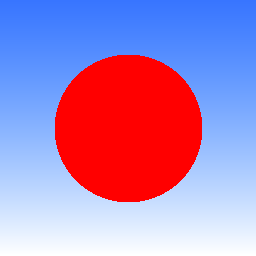
\includegraphics[width=0.5\textwidth]{media/firstSphere.png}
		\end{center}
	}<2>
\end{frame}

\begin{frame}[fragile]
	\frametitle{Making a Sphere Class}
	\begin{itemize}
		\item Sphere contains center, radius, color, and intersection method
	\end{itemize}
	\inputminted[fontsize=\footnotesize]{python}{scripts/sphereClass.py}
\end{frame}

\begin{frame}[fragile]
	\frametitle{Storing Intersection Information}
	\begin{itemize}
		\item Often require knowing a lot of information about intersection; for now we just have location and color, but in more robust renderers, it can store texture coordinates, information about the material, etc.
		\item Store the information in a \texttt{HitRecord} object
	\end{itemize}
	\inputminted{python}{scripts/HitRecord.py}
\end{frame}

\begin{frame}[fragile,t]
	\frametitle{Calculate Normal of Sphere}
	\begin{itemize}
		\item Normal is unit vector perpendicular to the surface
		\item For sphere, it's vector from center to point
	\end{itemize}
	\only{
		\begin{center}
			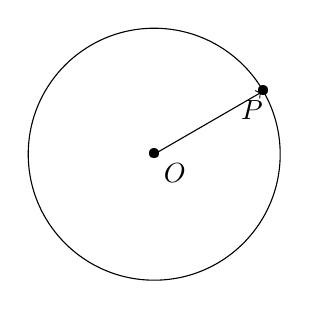
\begin{tikzpicture}[scale=0.4]
				\draw (0, 0) circle (4cm);
				\node at (0, 0) {\textbullet};
				\draw (0, 0) node [below right] {$O$};
				\node at (3.464101615, 2) {\textbullet};
				\draw (3.7541016, 2) node [below left] {$P$};
				\draw[->] (0, 0) -- (3.4067811, 1.97);
			\end{tikzpicture}
		\end{center}
	}<1>
	\begin{onlyenv}<2>
		\inputminted{python}{scripts/sphereNormal.py}
	\end{onlyenv}
\end{frame}

\begin{frame}[fragile]
	\frametitle{Updated Sphere Intersection}
	\begin{itemize}
		\item We can use the new \texttt{HitRecord} in the \texttt{Sphere} intersection method
	\end{itemize}
	\inputminted[fontsize=\small]{python}{scripts/updatedSphereIntersection.py}
\end{frame}

\begin{frame}[fragile]
	\frametitle{Rendering Multiple Spheres}
	\begin{itemize}
		\item Go through all spheres, find the one with smallest positive intersection time
		\item Return color associated with it
	\end{itemize}
	\inputminted[fontsize=\small]{python}{scripts/multipleSpheres.py}
\end{frame}

\begin{frame}[fragile]
	\frametitle{Rendering Multiple Spheres}
	\begin{itemize}
		\item Go through all spheres, find the one with smallest positive intersection time
		\item Return color associated with it
	\end{itemize}
	\begin{onlyenv}<1>
		\inputminted[fontsize=\small]{python}{scripts/multipleSpheres2.py}
	\end{onlyenv}
\end{frame}

\begin{frame}[fragile]
	\frametitle{Updating Scene}
	\begin{itemize}
		\item Make list of all the spheres in the scene
	\end{itemize}
	\begin{onlyenv}<1>
		\inputminted{python}{scripts/multipleLoop.py}
	\end{onlyenv}
	\only{
		\begin{center}
			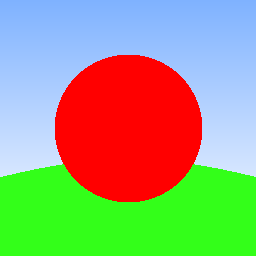
\includegraphics[width=0.5\textwidth]{media/multipleSpheres.png}
		\end{center}
	}<2>
\end{frame}

\section{Materials}

\begin{frame}
	\frametitle{Shading}
	\begin{itemize}
		\item So far, everything looks flat. How can we give the illusion of depth?
		\item Right now, light stops once it hits something, which isn't very realistic
		\item In real life, light bounces around until it is absorbed by something
		\item Even though our rays start at the camera, the same effect occurs
		\item Changing the way rays of light bounce changes how the material looks
	\end{itemize}
\end{frame}

\begin{frame}[fragile]
	\frametitle{Lambertian Material}
	\begin{itemize}
		\item Easiest material to simulate is called ''lambertian''; models rough surfaces, looks the same from all angles
		\item Need to generate new direction for a ray, for lambertian material this is done with generating a unit vector
	\end{itemize}
	\inputminted{python}{scripts/randSphere.py}
\end{frame}

\begin{frame}
	\frametitle{Generating new Ray Direction}
	\begin{itemize}
		\item Given normal $\vec{n}$ and randomly generated unit vector $\vec{d}$, the new direction is $\vec{n}+\vec{d}$
	\end{itemize}
	\begin{center}
		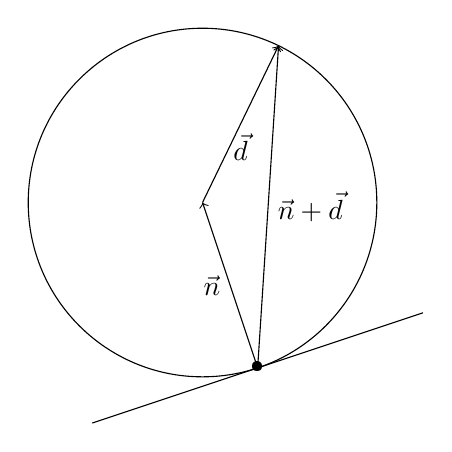
\begin{tikzpicture}[scale=0.7]
			\draw (0, 0) node {\textbullet};
			\draw[->] (0, 0) -- (-1, 3) node [midway,left] {$\vec{n}$};
			\draw (-1, 3) circle (3.16227766cm);
			\draw (-3, -1) -- (3, 1);
			\draw[->] (-1, 3) -- (0.3794838, 5.845527) node [midway,below] {$\vec{d}$};
			\draw[->] (0, 0) -- (0.3794838, 5.845527) node [midway,right] {$\vec{n} + \vec{d}$};
		\end{tikzpicture}
	\end{center}
\end{frame}

\begin{frame}[fragile]
	\frametitle{Updating \texttt{get\_intersection}}
	\begin{itemize}
		\item We must now store the depth of the traversal, how many bounces we've done, and eventually stop; call with arbitrary depth (like 20)
	\end{itemize}
	\inputminted[fontsize=\small]{python}{scripts/intersectionDepth.py}
\end{frame}

\begin{frame}
	\frametitle{Render with Shadows}
	\begin{itemize}
		\item Now the image has a lot of noise
		\item A single ray can't capture enough information to accurately estimate what the image should look like
		\item Increase accuracy by sending multiple rays per pixel
	\end{itemize}
	\begin{center}
		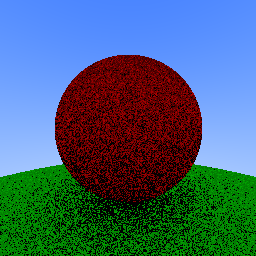
\includegraphics[width=0.45\textwidth]{media/shading.png}
	\end{center}
\end{frame}

\begin{frame}[fragile]
	\frametitle{Multiple Samples}
	\begin{itemize}
		\item Set color to average of all samples
		\item Taking $n$ samples per pixel makes render take $n$ times longer to finish
	\end{itemize}
	\begin{onlyenv}<1>
		\inputminted{python}{scripts/samples.py}
	\end{onlyenv}
	\only{
		\begin{center}
			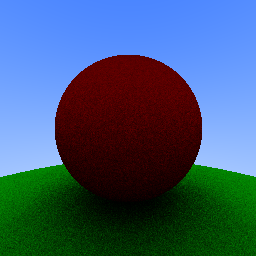
\includegraphics[width=0.5\textwidth]{media/samples.png}
		\end{center}
	}<2>
\end{frame}

\begin{frame}[fragile]
	\frametitle{Anti-Aliasing}
	\begin{itemize}
		\item Image still contains harsh boundaries between sphere and background
		\item Each pixel only contains what's at the center of the pixel
	\end{itemize}
	\begin{center}
		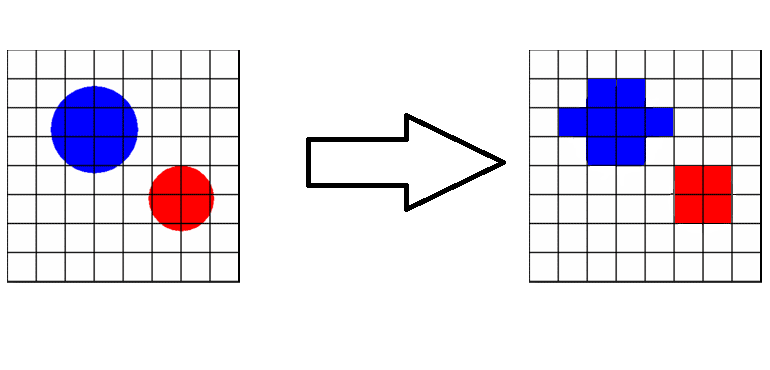
\includegraphics[width=0.8\textwidth]{media/aliasExample.png}
	\end{center}
	
\end{frame}
\begin{frame}[fragile]
	\frametitle{Anti-Aliasing}
	\begin{itemize}
		\item Nudging each original ray better represents what the pixel shows
	\end{itemize}
	\begin{onlyenv}<1>
		\inputminted[fontsize=\small]{python}{scripts/aliasing.py}
	\end{onlyenv}
	\only{
		\begin{columns}[T]
		\begin{column}{0.5\textwidth}
			\centering
			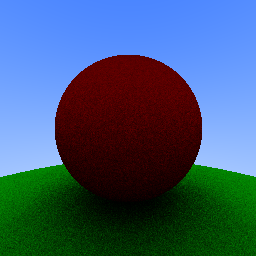
\includegraphics[width=\textwidth]{media/samples.png}
		\end{column}
		\begin{column}{0.5\textwidth}
			\centering
			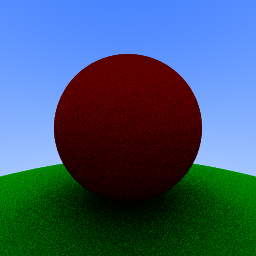
\includegraphics[width=\textwidth]{media/aliasing.png}
		\end{column}
	\end{columns}
	}<2>
\end{frame}

\begin{frame}[fragile]
	\frametitle{Lambertian Class}
	\begin{itemize}
		\item We want to eventually have multiple materials, so lets abstract the material into a class
		\item Stores the color and has single method to return new direction for ray
	\end{itemize}
	\inputminted{python}{scripts/lambertian.py}
\end{frame}

\begin{frame}[fragile]
	\frametitle{Updating Sphere Class}
	\begin{itemize}
		\item Sphere class now has a \texttt{material} member instead of \texttt{color}
	\end{itemize}
	\inputminted[fontsize=\footnotesize]{python}{scripts/newSphere.py}
\end{frame}

\begin{frame}[fragile]
	\frametitle{Updating HitRecord Class}
	\begin{itemize}
		\item Similarly, \texttt{HitRecord} now has a \texttt{material} member instead of \texttt{color}
	\end{itemize}
	\inputminted{python}{scripts/newRecord.py}
\end{frame}

\begin{frame}[fragile]
	\frametitle{Updating \texttt{get\_intersection} Method}
	\begin{itemize}
		\item Use \texttt{scatter} on the \texttt{material} in the \texttt{HitRecord} to get the new direction
	\end{itemize}
	\inputminted{python}{scripts/newGetIntersection.py}
\end{frame}

\begin{frame}[fragile]
	\frametitle{Updating Render Loop}
	\begin{itemize}
		\item Construct spheres using new \texttt{Lambertian} class
	\end{itemize}
	\inputminted{python}{scripts/newLoop.py}
\end{frame}

\begin{frame}
	\frametitle{Updating Render Loop}
	\begin{itemize}
		\item Resulting image is the same, but the code is more flexible
		\item This is the final scene rendered at 5,000 samples per pixel
	\end{itemize}
	\begin{center}
		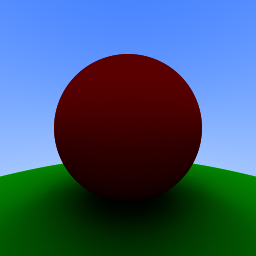
\includegraphics[width=0.5\textwidth]{media/final.png}
	\end{center}
\end{frame}

\section{Suggested Improvements and Resources}

\begin{frame}
	\frametitle{What next?}
	\begin{itemize}
		\item Implement reflective, metallic material (reflect ray about normal vector)
		\item Implement transparent glass-like material (refract ray using Snell's law)
		\item Modify the camera and use the \texttt{focal\_length} variable to create a depth-of-field effect
		\item Add texture coordinates so that you can wrap an image on a sphere
		\item Add support for more shapes
		\begin{itemize}
			\item If you add support for triangles, you can import meshes (\texttt{.obj} files) and render arbitrary objects
		\end{itemize}
		\item Make it multi-threaded (rendering is ``embarrassingly parallelizable'')
	\end{itemize}
\end{frame}

\begin{frame}
	\frametitle{Further Reading and Resources}
	
	\begin{itemize}
		\item Ray Tracing in a Weekend (\url{https://raytracing.github.io/})
		\begin{itemize}
			\item These slides are \textit{heavily} inspired by this series
		\end{itemize}
		\item Physically Based Rendering (\url{http://www.pbr-book.org/3ed-2018/contents.html})
		\begin{itemize}
			\item Very in-depth (sometimes too in-depth), but also very advanced and dense
		\end{itemize}
		\item Advanced Global Illumination, 2nd Edition
		\begin{itemize}
			\item Math-heavy, but also thorough (I'm currently reading this)
		\end{itemize}
		\item An in-depth look at a variety of materials (\url{https://blog.selfshadow.com/publications/s2013-shading-course/hoffman/s2013\_pbs\_physics\_math\_slides.pdf})
		\item List of websites with meshes that you can render:
		\begin{itemize}
			\item \url{https://casual-effects.com/data/}
			\item \url{https://threedscans.com/}
			\item \url{https://pbrt.org/scenes-v3.html}
		\end{itemize}
	\end{itemize}	
\end{frame}

\end{document}